\documentclass[a4paper]{jpconf}
\usepackage{graphicx}

\begin{document}
\title{AutoPyFactory: A Scalable Flexible Pilot Factory Implementation}

\author{J. Caballero$^1$, J. Hover$^1$, P. Love$^2$, G. A. Stewart$^3$ on behalf of the ATLAS Collaboration} 

\address{$^1$ Brookhaven National Laboratory, PO BOX 5000 Upton, NY 11973, USA}
\address{$^2$ Department of Physics, Lancaster University, Lancaster, LA1 4YB, UK}
\address{$^3$ CERN: European Organization for Nuclear Research, Geneva, Switzerland}

\ead{jcaballero@bnl.gov}

\begin{abstract}

The ATLAS experiment at the CERN LHC is one of the largest users of grid computing 
infrastructure, which is a central part of the experiment's computing operations.
Considerable efforts have been made to use grid technology in the most efficient
and effective way, including the use of a pilot job based workload management framework.
In this model the experiment submits 'pilot' jobs to sites without payload. When these
jobs begin to run they contact a central service to pick-up a real payload to execute.
The first generation of pilot factories were usually specific to a single Virtual Organization (VO), and were
bound to the particular architecture of that VO's distributed processing.
A second generation provides factories which are more flexible, not tied to any particular VO,
and provide new and improved features such as monitoring, logging, profiling, etc.
In this paper we describe this key part of the ATLAS pilot architecture, a second
generation pilot factory, AutoPyFactory.
AutoPyFactory has a modular design and is highly configurable. It is able to send
different types of pilots to sites and exploit different submission mechanisms and queue
characteristics. It is tightly integrated with the PanDA job submission framework,
coupling pilot flow to the amount of work the site has to run. It gathers information
from many sources in order to correctly configure itself for a site and its decision logic
can easily be updated.
Integrated into AutoPyFactory is a flexible system for delivering both generic and
specific job wrappers which can perform many useful actions before starting to run
end-user scientific applications, e.g., validation of the middleware, node profiling
and diagnostics, and monitoring.
AutoPyFactory also has a robust monitoring system that has been invaluable in establishing a
reliable pilot factory service for ATLAS.
\end{abstract}


\section{Introduction}

LHC experiments have adopted jobs workflows based on pilot systems.
Even though the particular implementation of these pilot-based architectures may
vary between different Virtual Organizations (VOs), the philosophy is the same. 
ATLAS [1] is one of the experiments using this pilot-based architecture.

Generic pilot jobs are submitted to sites without payload. 
When these jobs start on a worker node they contact a central VO
service to retrieve a real payload (i.e., an end-user job) and execute it.
Using these pilot-based workflows helps to improve job reliability,
optimize resource utilization, allows for opportunistic resources usage, 
and mitigates many of the problems associated with the inhomogeneities found on the grid [2].

Therefore, VOs need a reliable, robust and scalable
framework capable of managing the automatic flow of pilots to remote Grid
resources, conditional on the amount of work ready to be performed.
These pilot frameworks need to address the different policies that the VOs
implement to handle the different types of payload flavors.

AutoPyFactory is one of these pilot frameworks.


\section{Architecture}

AutoPyFactory runs in a single daemonized process,
launching a separate thread for each internal workflow (known as an APFQueue).
Each one of these APFQueues typically serves a single job queue 
as defined in the VO Workload Management Service (WMS), 
and delivers pilots to a single batch queue, either local or remote. 

The behavior of these AutoPyFactory workflows, or APFQueues,
is determined by the combination of a set of plug-ins, 
invoked in a fixed order, in a loop, each one in charge of the performance of a well defined action.

These steps can be summarized as follows:
\begin{itemize}
    \item Retrieves possible extra configuration information from an external source 
          and merges it with the one from the local configuration files.
    \item Inspects the VO WMS service to query for end-user jobs and their state.
    \item Inspects the submission system to query how many pilots are already running or still idle.
    \item Calculates a number of new pilots to submit based on that information.
    \item Submits as many new pilots as needed, determined by the previous step.
\end{itemize}

Those functions that are shared between more than one APFQueue, such
as querying the WMS or a local batch system,
are performed in a threaded object (implemented following the Singleton design
pattern), and their information is shared by multiple APFQuees. This approach
greatly reduces the load on those services and increases the reliability and performance of the whole system.

Figure 1 shows a diagram with the conceptual design and 
interactions between different components.

\begin{figure}[h]
\centering\includegraphics[width=0.85\textwidth]{apfdesign}
\caption{AutoPyFactory design}
\label{apfdesign}
\end{figure}

\subsection{AutoPyFactory internal nomenclature}

The communication between different modules in AutoPyFactory 
is possible thanks to its internal nomenclature:
a set of generic variables with a specific meaning which all components 
understand, allowing them to work together. 
Table 1 and Table 2 show the AutoPyFactory names for the
possible states in the batch submission system. 

\begin{table}[h]
   \begin{center}
      \begin{tabular}{l l}
         \hline
         \textbf{AutoPyFactory status} & \textbf{Description} \\ 
         \hline
         pending      &     job is queued (somewhere) but not running yet.      \\  
         running      &     job is currently active (run + stagein + stageout)  \\ 
         error        &     job has been reported to be in an error state       \\ 
         suspended    &     job is active, but held or suspended                \\ 
         done         &     job has completed                                   \\ 
         unknown      &     unknown or transient intermediate state             \\ 
         \hline
      \end{tabular}
   \end{center}
   \caption{Batch submit system primary AutoPyFactory job status}
   \label{job secondary status}
\end{table}

\begin{table}[h]
   \begin{center}
      \begin{tabular}{l l}
         \hline
         \textbf{AutoPyFactory status} & \textbf{Description}  \\ 
         \hline
         transferring  &     stagein + stageout  \\ 
         stagein       &                         \\ 
         stageout      &                         \\ 
         failed        &     (done - success)    \\ 
         success       &     (done - failed)     \\ 
         \hline
      \end{tabular}
   \end{center}
   \caption{Batch submit system secondary AutoPyFactory job status} 
   \label{job secondary status}
\end{table}

Table 3 shows the list of AutoPyFactory names and their meaning 
for the possible states in the WMS system.

\begin{table}[h]
   \begin{center}
      \begin{tabular}{l l}
         \hline
         \textbf{AutoPyFactory status} & \textbf{Description} \\
         \hline
         notready &     job created in the WMS service, but not ready yet for execution\\ 
         ready    &     job ready to be picked up and start execution                  \\ 
         running  &     job is currently running                                       \\ 
         done     &     job has finished with success                                  \\ 
         failed   &     job has finished with no success                               \\ 
         \hline
      \end{tabular}
   \end{center}
   \caption{WMS service AutoPyFactory job status}
   \label{wms job status}
\end{table}

\subsection{Plug-ins design}

AutoPyFactory can serve to different queues in different ways 
thanks to its modular design based on plug-ins. 
Plug-ins serve two purposes. 
They interact with the external services, like the VO WMS or the batch submission system,
and they translate the information retrieved by those services into the internal AutoPyFactory nomenclature.
There are currently 5 types of plug-ins:


\subsubsection{Configuration Plug-in:}

Retrieves extra configuration content from remote sources 
(as a URL with the actual configuration file, or a web service with an API providing for the configuration content)
and merges them with the local configuration content.
An example of a configuration plug-in is the one that queries the PanDA [3]
SchedConfig service for submission characteristics.


\subsubsection{WMS Status Plug-in:}
Queries the VO WMS system, 
retrieving information about the number of jobs in different status (ready, running, finished...) per queue.
This information is converted internally into the AutoPyFactory nomenclature.
An example of a WMS Status plug-in queries the PanDA API.
Another example is a plug-in querying a local Condor [4] pool and interpreting the
output as end-user jobs. This source of information is typically where 
how much work is ready to be done can be found, and therefore should trigger pilot
submission. 


Table 4 shows an example of mapping between the VO WMS service 
(PanDA in this case)
and the internal AutoPyFactory nomenclature.

\begin{table}[h]
   \begin{center}
      \begin{tabular}{l l}
         \hline
         \textbf{Panda Status} & \textbf{AutoPyFactory Status}       \\
         \hline
         pending       & notready  \\ 
         defined       & notready  \\ 
         assigned      & notready  \\ 
         waiting       & notready  \\ 
         activated     & ready     \\ 
         starting      & running   \\ 
         sent          & running   \\ 
         running       & running   \\ 
         holding       & running   \\ 
         transferring  & running   \\ 
         finished      & done      \\ 
         failed        & failed    \\ 
         cancelled     & failed    \\ 
         \hline
      \end{tabular}
   \end{center}
   \caption{Mapping between PanDA status and AutoPyFactory WMS job status}
   \label{translation}
\end{table}


\subsubsection{Batch Status Plug-in:}
Queries the batch system being used to submit the jobs (or pilots) to the grid resources,
to determine how many previously submitted jobs are already being executed and how many are still idle.
This information is used to avoid submitting an unnecessary number of extra jobs, 
which could cause bottlenecks, inefficiencies, and even impose severe loads on remote Grid services.
An example is a module querying the Condor queues.
Tables 5 and 6 show two examples of mappings between the external services
and the internal AutoPyFactory nomenclature.

\begin{table}[h]
   \begin{center}
      \begin{tabular}{l l}
         \hline
         \textbf{Condor Local Status}  & \textbf{AutoPyFactory Status}       \\ 
         \hline
         Unexpanded (the job has never run)    &  pending     \\
         Idle                                  &  pending     \\
         Running                               &  running     \\
         Removed                               &  done        \\
         Completed                             &  done        \\
         Held                                  &  suspended   \\
         Transferring Output                   &  running     \\
         \hline
      \end{tabular}
   \end{center}
   \caption{Mapping between Condor status and AutoPyFactory batch job status}
   \label{translation}
\end{table}

\begin{table}[h]
   \begin{center}
      \begin{tabular}{l l}
         \hline
         \textbf{Globus status Status}   & \textbf{AutoPyFactory status}       \\ 
         \hline
         PENDING       &   pending    \\
         ACTIVE        &   running    \\
         FAILED        &   done       \\
         DONE          &   done       \\
         SUSPENDED     &   suspended  \\
         UNSUBMITTED   &   pending    \\
         STAGE\_IN     &   running    \\
         STAGE\_OUT    &   running    \\
         \hline
      \end{tabular}
   \end{center}
   \caption{Mapping between globus status and AutoPyFactory batch job status}
   \label{translation}
\end{table}


\subsubsection{Scheduler Plug-in:}
This is the component in charge of making a decision of whether or not to submit
more pilots, and if so how many. That calculation is based on the information
provided by the two Status plug-ins (WMSStatus and BatchStatus).
It implements a given algorithm to decide how many new jobs (or pilots) should be submitted next cycle. 
A typical algorithm calculates the number of new jobs based on the number of end-user jobs in a ready status in the VO WMS service, 
with some constraints to prevent the submission of an excessively high number of jobs, 
or to eventually keep a minimum number of submissions per cycle. 
Figure 2 shows the logical flow implemented in the
ActivatedSchedPlugin (so named because it is primarily keyed on the number of
ready jobs in the WMS). Other SchedPlugins may embody other algorithms, e.g. a
scheduler plug-in could always return a fixed number of jobs, or one could seek
to maintain a constant number of pending/queued jobs in the batch system. 

\begin{figure}
\centering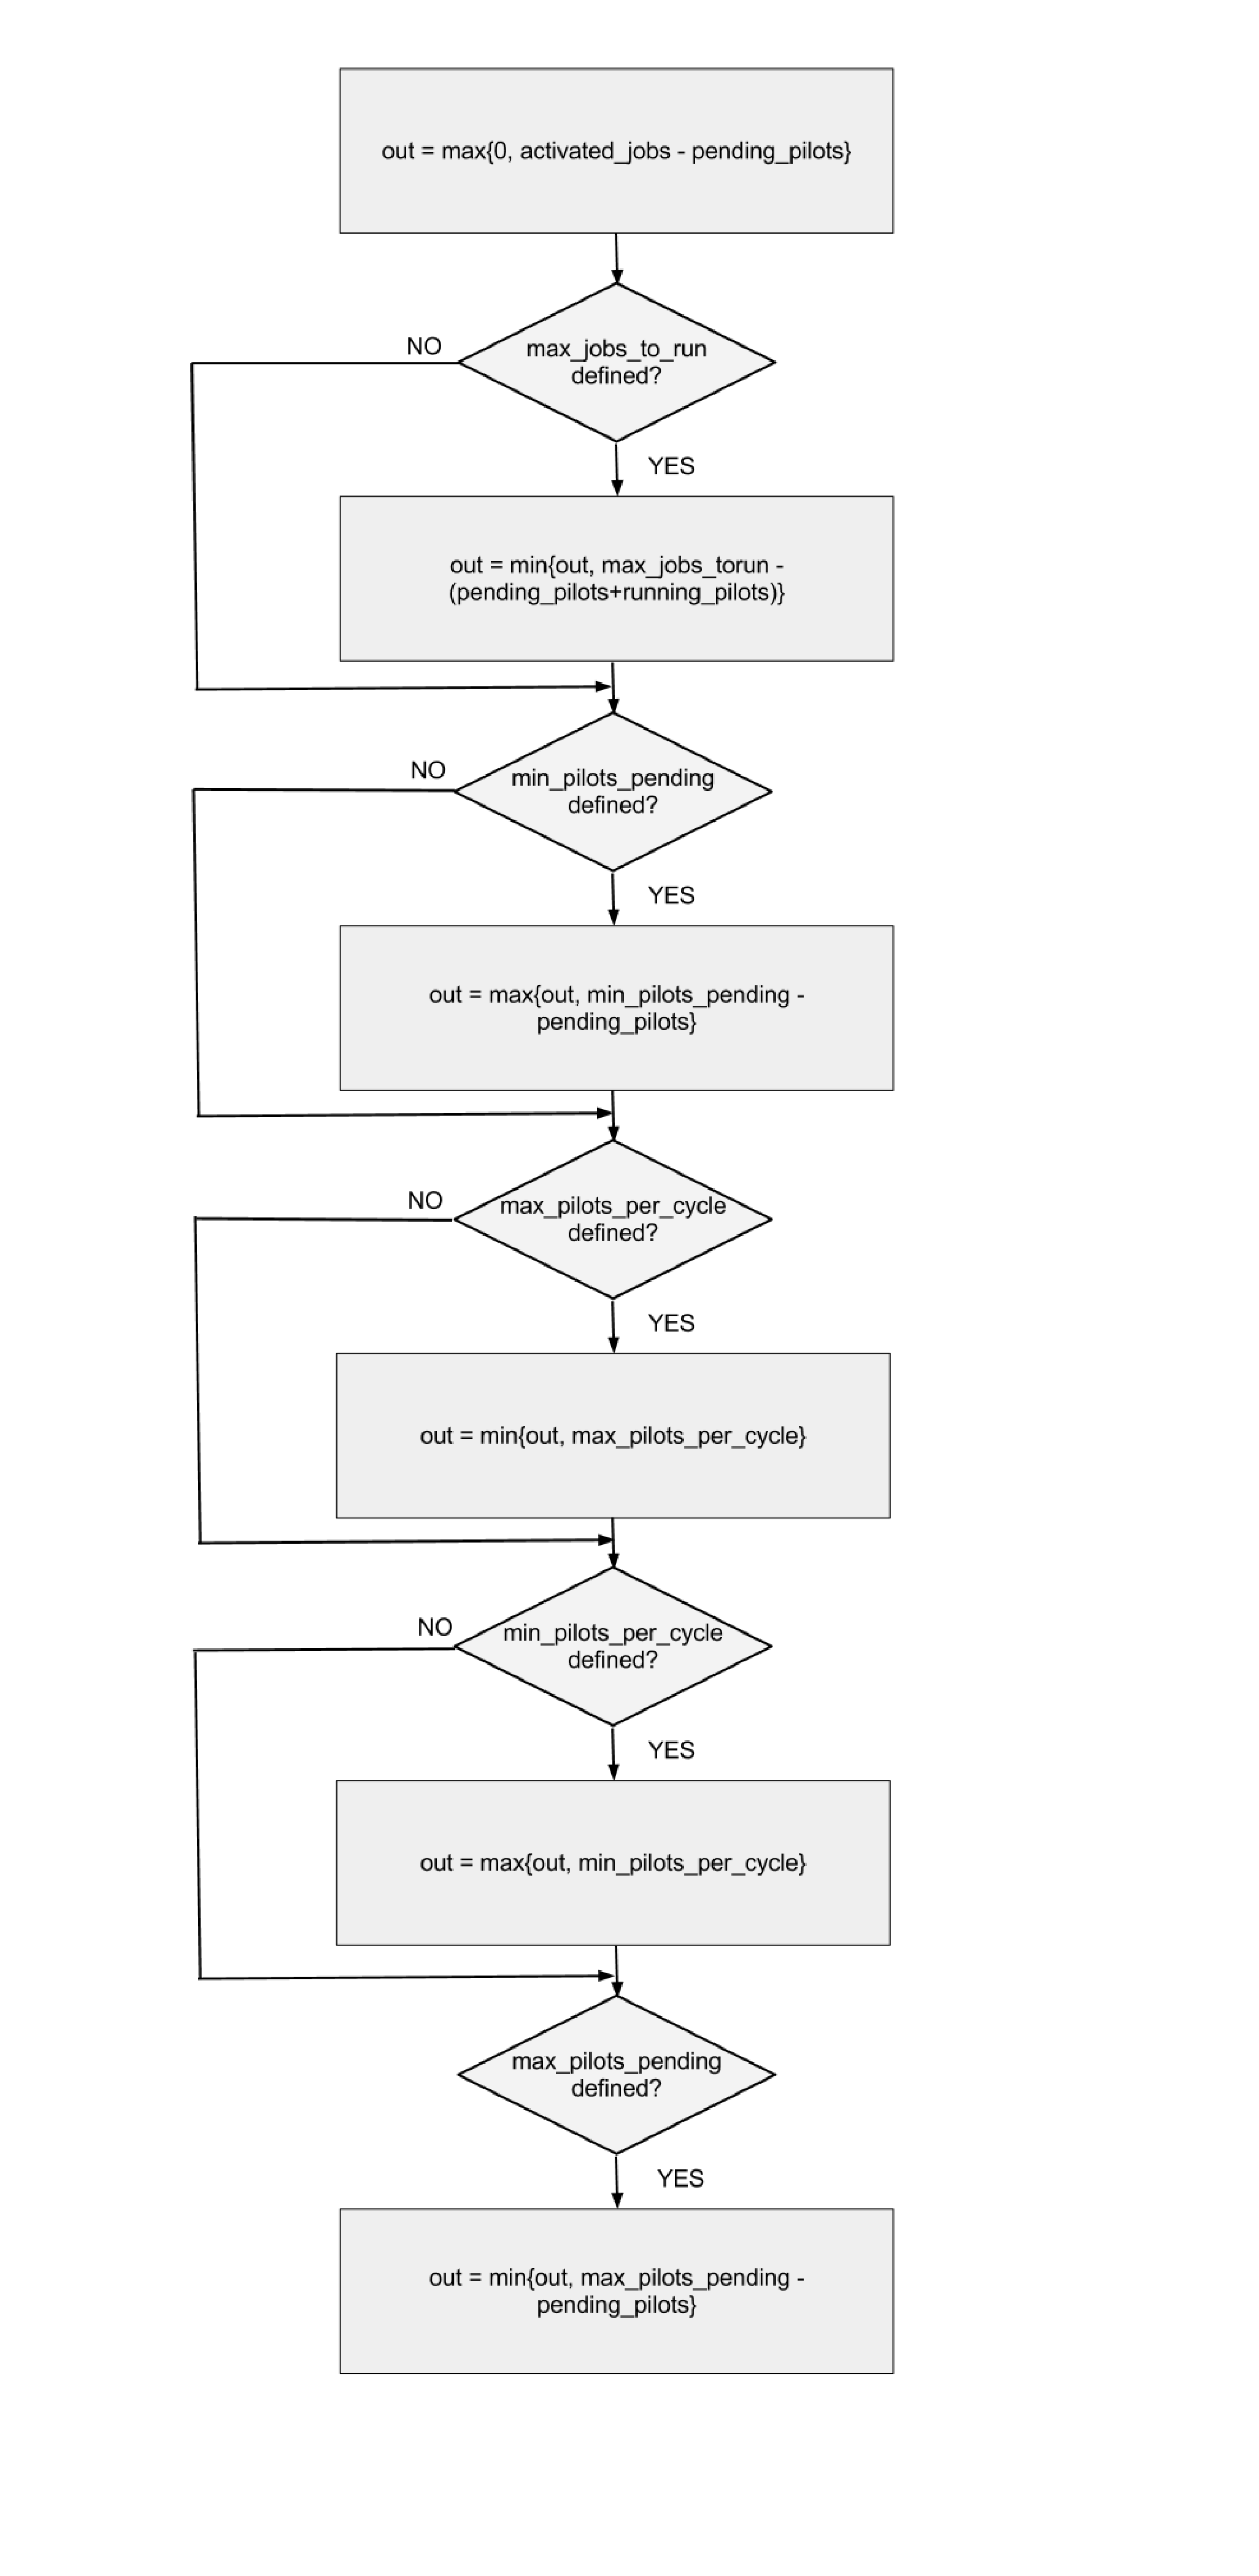
\includegraphics[width=0.7\textwidth]{activated}
\caption{Activated algorithm}
\label{activatedfigure}
\end{figure}

\subsubsection{BatchSubmit Plug-in:}
It is the component in charge of submitting new jobs (or pilots), 
based on the decision made by the Scheduler plug-in. 
Examples of these execution plug-ins can submit jobs remotely to a Grid resource using different protocols 
(such as GRAM2, GRAM5, or CREAM), to a Cloud Computing resource 
(using the Amazon EC2 protocol), or to a local Condor pool. 

In theory, a submit plug-in
could use other mechanisms, e.g. simply execute a pilot process, or trigger an
additional VM startup locally via libvirtd. In this scenario, AutoPyFactory could be run
directly on the working resource (wherever the jobs are intended to run).


\subsection{Usage}

The normal usage, as explained above, 
makes use of a single set of 5 plug-ins per workflow. 
Typically, each APFQueue will serve one queue as it is defined in the WMS service, 
and will submit pilots to a queue as defined in the batch system. 
This allows for many-to-many combinations, each one served by one APFQueue in a single thread. 

However, more complex workflows can be achieved by the combination of two APFQueues working together.

\subsubsection{Cloud Computing with AutoPyFactory:}
The combination of two APFQueues, 
as it is shown in figure 3, 
can allow using Cloud Computing resources. 
For this to happen, the configuration of both APFQueues is like this:

\begin{itemize}
\item First APFQueue: 
The WMS Status plug-in queries the VO WMS service, and the Execution Plugin
submits jobs  to a local Condor pool.
This Condor pool can have many Worker Nodes, or zero. 
In the latter case, all submitted jobs will remain in idle status. 
\item Second APFQueue: 
the WMS Status plug-in queries this local Condor pool, 
and gives to idle jobs in the queue the same meaning that jobs ready in a VO WMS service have.
The Execution Plug-in then submits Virtual Machine instantiation orders (to an Amazon EC2-like resource, for example). 
The middleware pre-installed on these Virtual Machines, 
beside Grid middleware and any particular libraries required by the VOs, 
can include a Condor startd daemon which will join the local Condor pool. 
Once these remote instances have joined the Condor pool, 
the idle jobs will flow and start execution. 
\end{itemize}

\begin{figure}[h]
\centering\includegraphics[width=0.7\textwidth]{cloud}
\caption{Cloud Computing with AutoPyFactory}
\label{cloud}
\end{figure}

\subsubsection{Glideins submission with AutoPyFactory:}
It would be possible to replicate the above mechanism to allow Condor glideins submission with AutoPyFactory.
The architecture is similar, with two AutoPyFactory workflows combined.
The first one queries the VO WMS service and submits the jobs (or pilot) to the local pool, 
while the second one submits glideins to remote resources which will join that local pool. 

In theory, AutoPyFactory is flexible enough that it can serve new needs by mixing the
roles played by different plug-ins in whatever way accomplishes the required goal. 

\section{Monitor}

If desired, factory activity can be displayed in a central web based monitor,
which delivers some useful metrics and displays links to the particular job log
files. Figure 4 shows a diagram with the design of this monitor component.
The application uses the Django web framework with a mysql backend and apache webserver. 
The web service collects information from a number of
factories and allows a global view of Factory deployment with broad
views from Factory level to fine-grained information about individual pilot jobs. 
At 60k jobs created per hour, and over 2 million web hits per day, 
the monitoring stack must be tuned to prevent overloading.
The deployment of memcached has helped greatly in this respect.


\begin{figure}[h]
\centering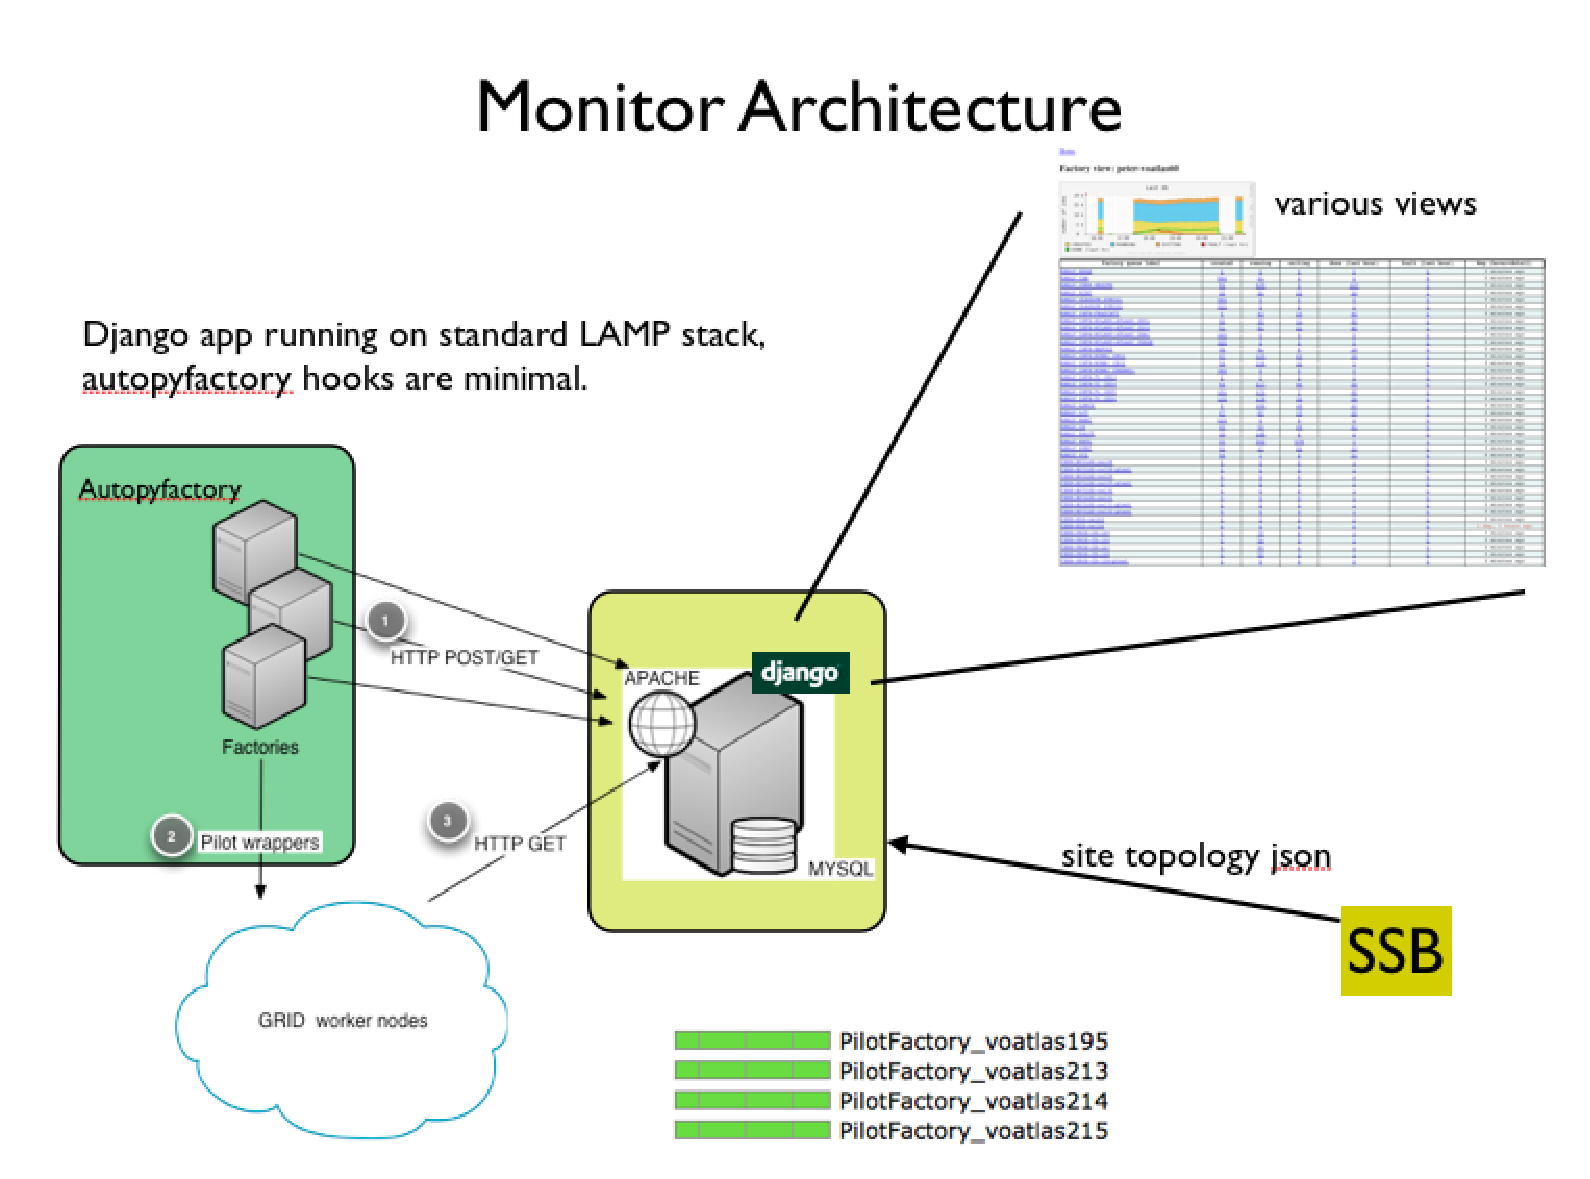
\includegraphics[width=0.7\textwidth]{monitor}
\caption{Monitor}
\label{monitor}
\end{figure}

\section{Proxy Manager}

For submission of pilots via the Grid, AutoPyFactory provides an integrated utility for
defining one or more grid or VOMS proxies to be generated and maintained while
the factory is running. Individual AutoPyFactory queues are configured to use whatever
proxy is appropriate. 


\section{Log Server}

AutoPyFactory includes the ability to export local directories via a built-in web server
configured within the factory. This is normally used to allow job log files to
be viewed remotely via links in the monitor. But any information that is
generated by an integrated component could be exported the same way. For
example, the Condor submit file can be examined via the web server as well. 


\section{Deployment}

\subsection{Packaging}
One of the goals of the development of AutoPyFactory was to allow for the possibility of
site administrators to install the pilot factory locally at their sites. They
would then submit pilots directly into their local batch system, rather than
relying on central pilot submission via Grid interfaces. 
Toward that end, AutoPyFactory has been made as easy to deploy as possible. 

AutoPyFactory is provided in the prevailing standard, versioned package format (RPM) and
made available using standard package management tools (yum). Signed yum
repositories (development, testing, and production) are maintained by the
developers and are available globally. This permits the easy installation and
upgrade of AutoPyFactory, either manually or via automation. 

This is useful beyond the usual deployment scenarios, e.g. one could dynamically
install AutoPyFactory as a pilot tool directly on virtual machines running in a Cloud
context. 

\subsection{UNIX Integration}
The infrastructure surrounding the AutoPyFactory runtime is made to be intuitive to
manage by systems administrators. By default, it is configured via conventional
Python ConfigParser-format files in /etc/apf (factory.conf, proxy.conf,
queues.conf) and /etc/sysconfig/factory. It can be started and stopped via the
standard init script in /etc/init.d. Factory logs are managed via the standard
Linux logrotate facility. 

\section{Future Steps}

As AutoPyFactory is fully modular and programmatically configurable, it is a candidate for
embedding within other frameworks. For example, a graphic Web user interface for
queue definition and management could be easily created on top of the existing
utility. 

AutoPyFactory is already being run in a semi-clustered way, with several instances all
identically configured. In this mode each of three servers, for example, handles
one third of submission load for each queue. If one of the nodes is lost, the
other two will naturally respond by increasing submissions (although the
individual jobs handled by the lost node will likely be lost). With the proper
approach, it would be feasible for AutoPyFactory to be enhanced to provide full fault
tolerance, such that clustered instances would be aware of each other directly,
or by way of flags placed in a global location or service. 

Currently AutoPyFactory makes decisions based on the instantaneous state of WMS and Batch
status information. In theory, adding persistence would allow submission
decisions made by the SchedPlugin to be even more intelligent, e.g. responding
to dynamic trends over the previous hours or days. Such a mechanism would also
allow the gathering of information over time, e.g. the maximum number of jobs
ever run at a site, which would allow a more intelligent ramp up strategy. 



%%\section{Acknowledgements}
\ack{
The authors are grateful for the contributions from all site system administrators who have tested the software
and have provided useful feedback to improve the software and its documentation: 
Doug Benjamin, Sarah Williams, Asoka da Silva.
}

\section*{References}
\begin{thebibliography}{99}

%\item LHC Computing Grid Project
%      {\it http://www.cern.ch/lcg/}

\item ATLAS Collaboration 1994 ATLAS Technical Proposal 
      {\it CERN/LHCC/94-43} 

\item Foster I, Kesselman C and Tuecke S 2001 The Anatomy of the Grid: Enabling Scalable Virtual Organizations
      {\it International J. Supercomputer Applications} {\bf 15}(3)

\item Nilsson P, Caballero J, De K, Maeno T, Potekhin M and Wenaus T 2008 The PanDA system in the ATLAS experiment
      {\it Proceedings of ACAT 2008 Conference.}

\item Douglas T, Todd T, and Miron L 2003 Condor and the Grid
      {\it Grid Computing: Making The Global Infrastructure a Reality, John Wiley}

\end{thebibliography}

~

%%Notice:
%%This manuscript has been authored by employees of Brookhaven Science Associates, 
%%LLC under Contract No. XXXXXXXXXX with the U.S. Department of Energy. 
%%The publisher by accepting the manuscript for publication acknowledges 
%%that the United States Government retains a non-exclusive, paid-up, irrevocable, 
%%world-wide license to publish or reproduce the published form of this manuscript, 
%%or allow others to do so, for United States Government purposes.

\end{document}

